\chapter{面向多中心用户的流行度预测方法}
\label{chap:four}
\section{引言}
社交网络已经成为人们日常生活中重要的一部分。随着时间的推移和互联网技术的发展,社交网络的功能和角色也发生了很大的变化。社交网络早期的主要功能是帮助用户在线上维护社交关系。用户可以在平台中发布自身的状态,同时也可以获取到自己关注的好友的状态信息。而当下的社交网络,更多地是在扮演着媒体的角色。从内容上看,用户在社交网络发布的内容,除却自身的状态更新外,更多地涉及当下的新闻和时事。大部分传统媒体也都直接在社交网络平台中开通了账号,便于第一时间发布各类消息。从结构上看,社交网络平台中的好友或关注机制,更多地在扮演订阅的角色。用户通过关注或者好友机制,从其他用户中获取自己感兴趣的内容。随着社交网络平台的媒体功能不断发展,进一步诞生了社交媒体的概念。借助于社交网络平台的优势,信息在社交媒体中传播地更快、更广,因此也吸引了研究者的广泛关注。

社交媒体中信息的传播模式与传统媒体有着很大的区别。在以门户网站、报纸、广播电视等为代表的传统媒体中,信息的传播都是中心式结构的:媒体是主要的发布内容者,也是用户获取信息的主要渠道,而社交媒体中信息的传播则呈现出一种去中心化的结构:信息在社交媒体中主要是沿着社交网络传播的。当用户发布信息后,他的粉丝就可以选择转发他的信息。在转发过程中,部分中间用户可能会累积大量的转发,进而使得整体的传播过程呈现出一种去中心化的结构。图\ref{fig:retweetExam}展示了新浪微博中一条消息的转发示意图,图中的每一个节点代表一个用户,每条边表示了对应用户间的转发关系。从图中可以看出,在转发过程中,有多个中间用户也累积了大量的转发,消息的整体传播结构呈现出去中心化的特点。这种去中心化的传播结构,为消息的传播预测带来了极大的挑战。
\begin{figure}[!htbp]
  \centering
  \includegraphics[width=1\textwidth]{4-retweetExam}
  \caption{新浪微博中消息的传播示例图}
  \label{fig:retweetExam}
\end{figure}

现有的用于刻画传播过程的模型主要包括基于自增强泊松过程的模型\citep{shen2014modeling,gao2015modeling}和基于自激励Hawkes过程的模型\citep{bao2015modeling,zhao2015seismic},但是这两类模型在社交媒体中刻画消息的传播过程时,都存在着各自的缺陷。基于自增强泊松过程的模型将消息的传播过程形式化为一个单源传播的过程,但是这一假设并不符合社交媒体中消息去中心化的传播模式,而且该类模型在建模每次转发带来的激励作用时,只是简单地统计消息的转发数,而没有对转发激励的大小进行区分。基于自激励Hawkes过程的模型建模了每次转发带来的激励作用,但是它需要为每一次转发学习一个激励参数,使得模型的参数学习在实际应用中难以实现,需要对模型做进一步的约减,进而影响了模型的预测能力。因此,我们仍然缺乏一个有效的用于刻画去中心化传播过程的方法。

我们对消息的传播过程进行了进一步的分析和研究,结果如图\ref{fig:multiCenter}所示。从图\ref{fig:multiCenter}(A)中可以看到,
\begin{figure}[!htbp]
  \centering
  \includegraphics[width=1\textwidth]{4-multiCenter}
  \caption{示例消息的多中心建模}
  \label{fig:multiCenter}
\end{figure}
消息整体的传播过程可以拆分为几个单源传播过程的叠加。我们将这几个单源传播过程的中心称为中心用户,并将中心用户引发的转发称为子过程。我们按照传播过程中的中心用户,将图\ref{fig:multiCenter}(A)中的传播过程拆分为6个单源传播子过程。在建模每个子过程时,我们选取了Shen等人提出的基于自增强泊松过程的RPP模型。RPP模型被提出用于解决论文引用数预测问题,非常适合单源传播的场景。RPP模型对6个子过程的建模结果如图\ref{fig:multiCenter}(B)所示。从图中可以看到,RPP模型可以很好地刻画每个中心用户引发的传播子过程。最后,我们将这6个RPP模型的预测结果按照时间顺序叠加,得到的流行度变化曲线与真实的流行度变化曲线非常相近。因此,通过叠加多个子过程来实现对消息整体传播过程的预测,是一种有效的方法。

在本章中,我们提出了一种基于RPP模型叠加的方法来刻画去中心化的传播过程。我们使用RPP模型来建模每个传播子过程,再将所有的传播子过程叠加,得到整体传播过程的建模。与基于自增强泊松过程的模型相比,我们的模型能够很好地捕获传播过程去中心化的特点,同时也区分了中心用户与其他转发用户带来的激励作用的差异;与基于自激励Hawkes过程的模型相比,我们的模型只需要学习中心用户的参数,大大减少了待学习的参数个数。

\section{数据分析}
我们在新浪微博上随机抓取了200条消息的完整转发数据,包括了转发用户、转发时间以及详细的转发路径数据,用于分析微博中的去中心化传播现象。我们从中随机挑选了几条消息的转发路径图,如图\ref{fig:diffusionTree}所示。图中的每一个点表示一条消息,消息之间的有向连边表示转发关系。我们将消息转发树中的第一个节点称为源发消息,其余节点称为转发消息。图\ref{fig:exampleD}展示是典型的中心型结构,所有消息基本上都是对源发消息的直接转发;图\ref{fig:exampleB}也是中心型的传播结构,只是部分传播链会比较长,但是没有其他消息得到大量的转发;图\ref{fig:exampleA}和图\ref{fig:exampleC}则展示了典型的去中心化结构。除源发信息外,部分转发消息本身也吸引了大量的传播,从而形成了一种多中心的传播结构。这种多中心的传播结构,目前还缺乏有效的建模方法,也是本章的建模目标。
\begin{figure}[!htb]
  \centering
  \begin{subfigure}[b]{0.4\textwidth}
    \includegraphics[width=\textwidth]{4-exampleA}
    \caption{}
    \label{fig:exampleA}
  \end{subfigure}%
  \hspace{0.05\textwidth}
  \begin{subfigure}[b]{0.4\textwidth}
    \includegraphics[width=\textwidth]{4-exampleB}
    \caption{}
    \label{fig:exampleB}
  \end{subfigure}
  \begin{subfigure}[b]{0.4\textwidth}
    \includegraphics[width=\textwidth]{4-exampleC}
    \caption{}
    \label{fig:exampleC}
  \end{subfigure}%
  \hspace{0.05\textwidth}
  \begin{subfigure}[b]{0.4\textwidth}
    \includegraphics[width=\textwidth]{4-exampleD}
    \caption{}
    \label{fig:exampleD}
  \end{subfigure}
  \caption{新浪微博中消息转发树示例}
  \label{fig:diffusionTree}
\end{figure}

为了进一步衡量微博中去中心化传播现象的比例,我们抓取了新浪微博中某一天所有的源发消息,以及这些源发消息在发布后24小时内的转发数据作为我们的实验数据。为了保证后续实验的效果,我们对数据进行了进一步的过滤。我们过滤了在发布1小时后累计转发数小于10的消息。最终我们的数据集中包含了近6.5万条源发消息以及它们的转发数据。

我们首先对源发消息的转发数据进行了统计。对于每一条源发消息,我们统计了它自身被直接转发的次数占总转发次数的比例,结果如图\ref{fig:rootRatioA}所示。图中横坐标是源发消息被直接转发的次数占消息最终总转发次数的比例,而纵坐标是转发比例小于等于对应横坐标比例的源发消息的累积分布。从图\ref{fig:rootRatioA}中可以看出,有接近20\%的消息的直接转发占总转发数的比例低于50\%,而接近50\%的消息的直接转发占总转发数的比例低于80\%,这说明直接将微博中的消息转发行为建模成单源传播是不合理的。为了消息低转发数消息对统计结果的影响,我们从数据集中剔除了最终转发数小于100的消息,并对剔除这些消息后得到的数据集进行统计,得到的统计结果如图\ref{fig:rootRatioB}所示。从图中可以看出,对于高转发数的消息来说,同样存在一定比例的源发消息,它们的直接转发占比比较低。
\begin{figure}[!htbp]
  \centering
  \begin{subfigure}[b]{0.5\textwidth}
    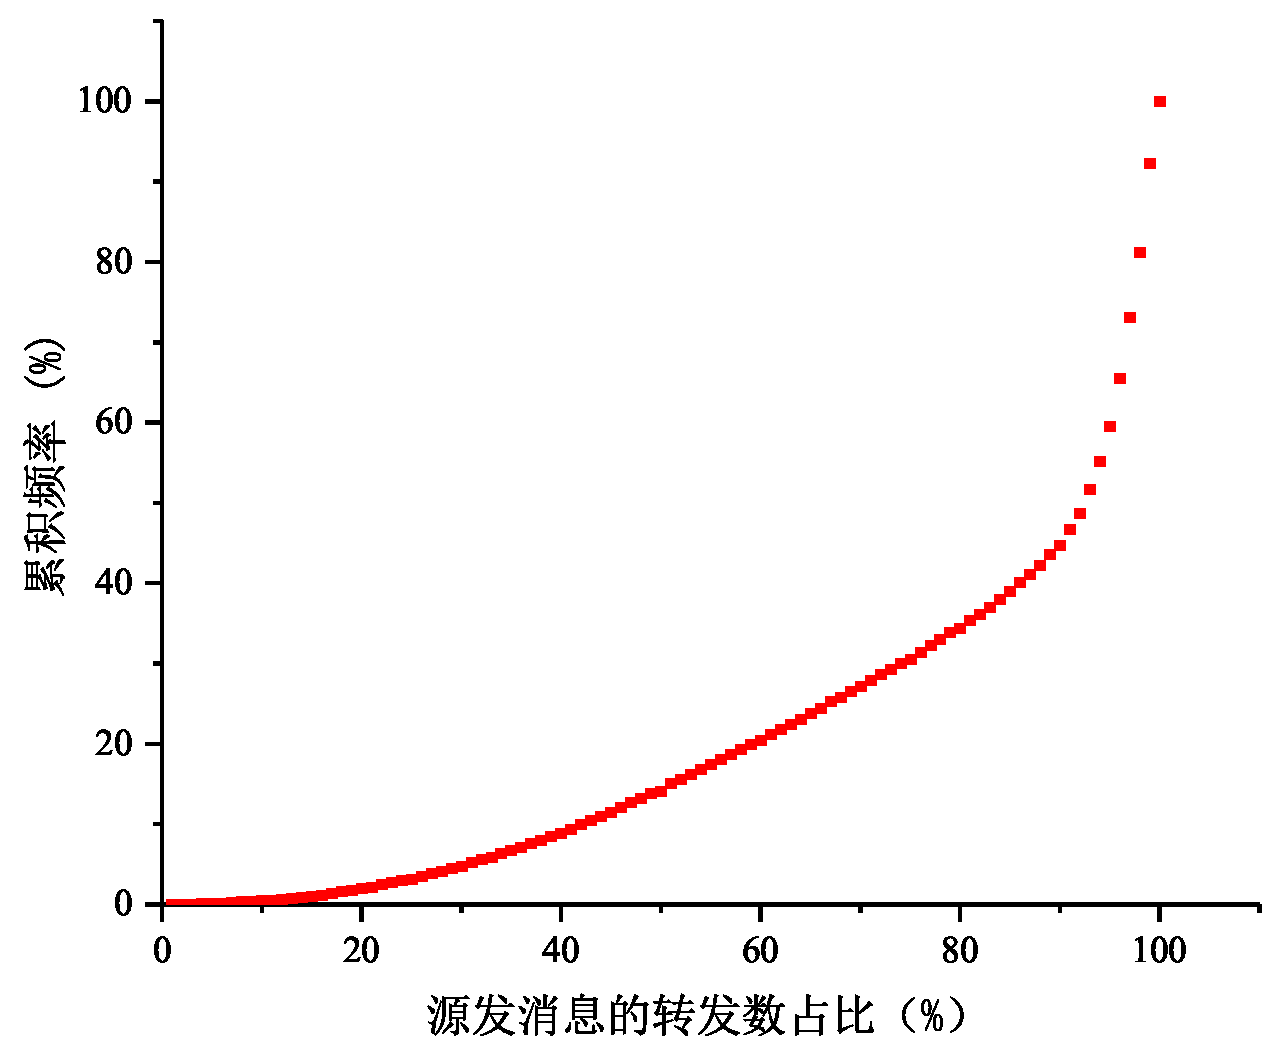
\includegraphics[width=\textwidth]{4-rootRatio}
    \caption{}
    \label{fig:rootRatioA}
  \end{subfigure}%
  \begin{subfigure}[b]{0.5\textwidth}
    \includegraphics[width=\textwidth]{4-rootRatioH}
    \caption{}
    \label{fig:rootRatioB}
  \end{subfigure}
  \caption{新浪微博中消息转发树示例}
  \label{fig:rootRatio}
\end{figure}

进一步地,我们统计了每条源发消息的转发消息引起的转发情况。对于每一条源发消息,我们搜集了它的所有的直接转发消息,统计了这些直接转发消息带来的转发数,并选取了这些直接转发消息中带来转发数最多的直接转发消息。我们统计了所选取的直接转发消息的转发数占源发消息总转发数的比例,得到的累积分布如图\ref{fig:burstRationH}所示。这里我们展示的是在剔除低转发数消息之后的数据集上的统计结果。从图中可以看出,有10\%的源发消息的直接转发消息带来的转发数占总转发数的比例超过了50\%,有20\%的源发消息的直接转发消息带来的转发数占总转发数的比例超过了30\%。这些统计结果说明,消息在传播过程中,除源发消息外还会出现少量引起大量转发的中间转发消息,对这些中间转发消息引起的转发情况的建模,是刻画去中心化传播过程的关键。
\begin{figure}[!htbp]
  \centering
  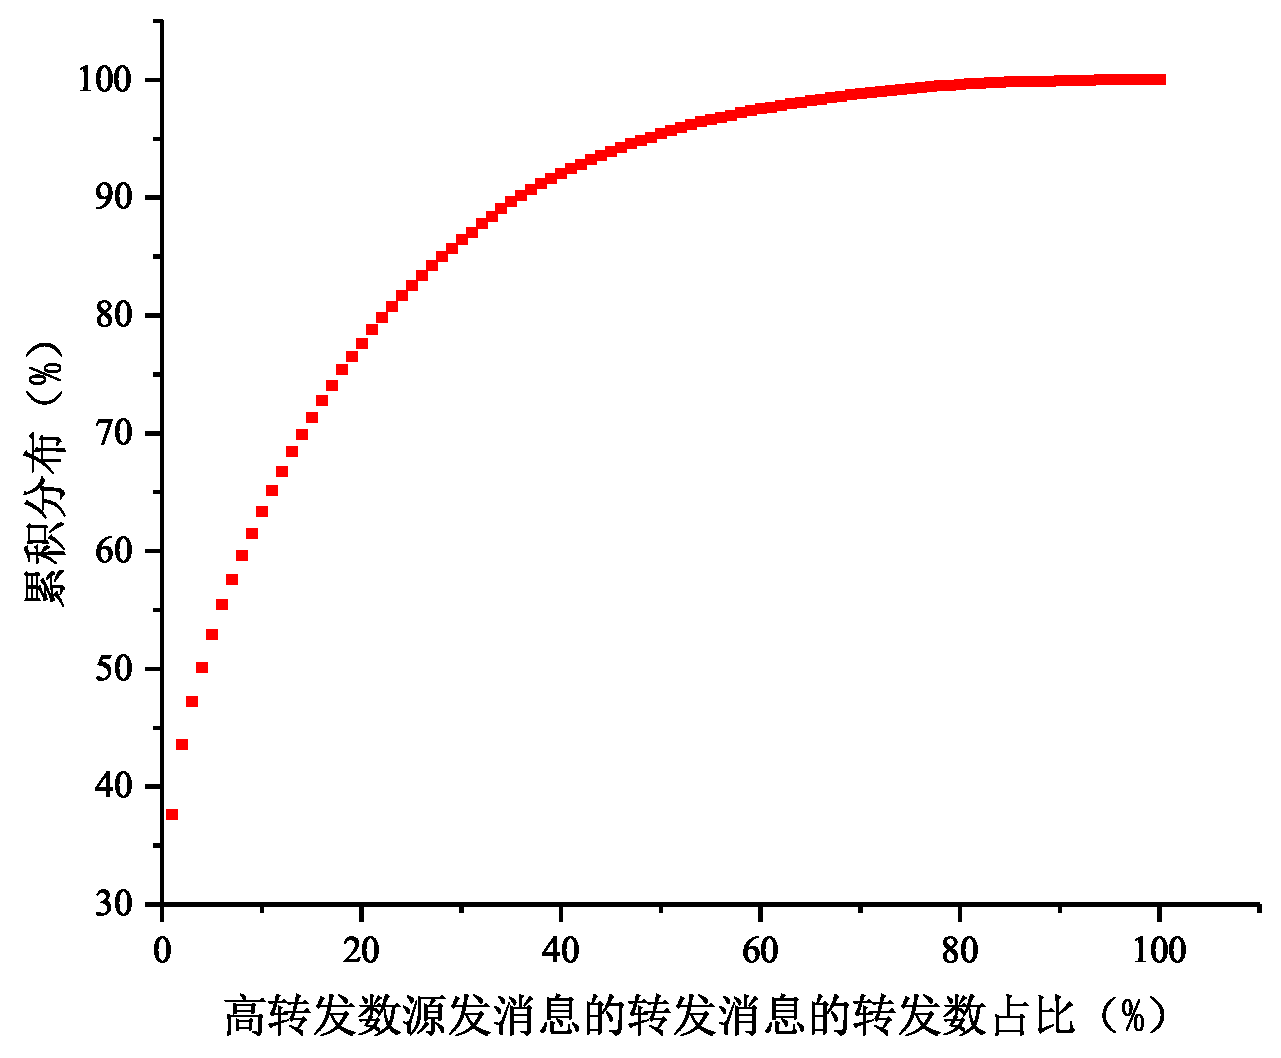
\includegraphics[width=0.5\textwidth]{4-burstRatioH}
  \caption{源发消息的转发消息引起的转发数的占比情况}
  \label{fig:burstRationH}
\end{figure}

综上所述,通过对数据集中消息的转发情况的分析,我们可以看出,去中心化的传播结构在消息传播过程中比较普遍,因此,我们需要一种模型来刻画去中心化的传播过程。进一步对各层转发消息的转发数据进行统计后发现,部分源发消息带来的直接转发数占比比较低,而部分转发消息则会带来很高的转发量。因此,刻画这些转发消息所引发的转发过程,是刻画去中心化传播过程的关键。

\section{模型}
\subsection{问题形式化}
给定一条消息$d$在观测时间窗口$[0,T]$内的转发时间戳序列$C^d=\{t_i^d|t_i^d<T,i=0,1,2,...,n_d\}$,其中$n_d$在消息$d$观测时间窗口内的转发次数,$t_i^d$是消息$d$的发布时间与第$i$次转发的时间的间隔,且满足$0=t_0^d \le t_1^d \le t_2^d \le...\le t_{n_i}^d \le T$。我们的目标是预测消息$d$在后续任意时刻$t$的转发数。

\subsection{RPP模型}
RPP模型是由Shen等人提出并被用于建模论文引用数的到达过程,它是一个基于随机过程的模型。关于基于随机过程的模型的相关知识,可以参考本论文的第二章相关研究综述中的相关内容。RPP模型在建模论文的引用达到过程时,重点考虑了3个影响论文引用数的因素:首先是论文本身的质量因素。论文的质量越高,论文的最终引用数会越高,而且引用数增长的速度也越快。第二个因素是时间衰减效应。类似于信息传播中的爆发衰减现象,论文引用数的增长也同样会存在爆发阶段和衰减阶段,需要利用一个时间函数来刻画论文的引用增长速度随时间的变化过程。最后一个因素是论文引用中的``富者愈富"机制\citep{jeong2003measuring,wang2008measuring}。在论文引用过程中,引用数越高的论文,越有机会获得更多新的引用。Shen等人使用了乘性模型来融合上述3个因素,最终给出了如下的论文引用强度函数:
\begin{equation}
\label{eq:rppDiff}
\frac{dc(t)}{dt}=x(t)=\lambda f(t;\theta) I(t)\text{,}
\end{equation}
其中$c(t)$是到$t$时刻论文的总引用数。$\lambda$用于度量论文的质量;$f(t;\theta)$用于刻画时间衰减效应,$\theta$是对应的参数。在RPP模型中,作者选用的时间衰减效应函数是Log-normal函数;$I(t)$用于刻画论文累积引用数带来的``富者愈富"影响。在RPP模型中,$I(t)$函数的值就是到$t$时刻为止论文的累积引用数,即$I(t)=m+c(t)$,其中$m$是作者引入的论文引用数的先验。在给定强度函数后,就可以利用极大似然框架来求取相应的参数。类似于前面定义的时间戳序列,论文引用序列也可以用$\{t_0,t_1,t_2,...,t_N\}$表示,其中$t_i$是第$i$引用的到达时刻与论文发表时刻的时间间隔,$N$是论文的总引用次数。利用第二章相关工作综述中介绍的生存理论分析框架,论文引用序列的似然函数可以表示为:
\begin{equation}
L(\lambda,\theta)=p_0(T|t_N)\prod_{i=1}^{N}p_1(t_i|t_{i-1})\text{,}
\end{equation}
其中$p_0(T|t_N)$表示时间区间$(t_N, T]$内没有新的引用到达的概率。在生存理论分析框架中,给定强度函数$x(t)$后,时间区间$(t_N, T]$内没有新的引用到达的概率可以用生存概率建模如下:
\begin{equation}
p_0(T|t_N)=e^{-\int_{t_N}^{T}x(t_N)dt}=e^{-\int_{t_N}^{T}\lambda f(t;\theta) I(t_N)dt}\text{;}
\end{equation}
$p_1(t_i|t_{i-1})$表示了在给定前一次引用发生在$t_{i-1}$时刻的情况下,下一次引用发生在$t_i$时刻的概率密度。在生存理论分析框架中,这个概率密度为:
\begin{equation}
p_1(t_i|t_{i-1})=x(t_{i-1})e^{-\int_{t_{i-1}}^{t_i}x(t_{i-1})dt}=\lambda f(t;\theta) I(t_{i-1})e^{-\int_{t_{i-1}}^{t_i}\lambda f(t;\theta) I(t_{i-1})dt}\text{。}
\end{equation}
给定上述定义后,结合观测数据,就可以利用极大似然框架来推断强度函数中的相应参数,进而对论文引用数的后续变化进行预测。假设估计得到的参数为$\{\lambda^{\ast},\theta^{\ast}\}$,通过求解微分方程(\ref{eq:rppDiff}),并结合边界条件$c(T)=N$,论文在$t$时刻的引用数可以用如下函数预测:
\begin{equation}
c(t)=(m+N)e^{\lambda^{\ast}\int_{T}^{t}f(t;\theta^{\ast})dt}-m\text{。}
\end{equation}

RPP模型在预测论文引用数变化时,取得了非常好的效果。但是论文引用场景更像是一个单源传播的场景,而消息传播则呈现出明显的多中心结构。因此,本章提出了一种面向多中心用户的流行度到达过程建模方法。
\subsection{面向多中心用户的流行度到达过程建模}
通过数据分析,我们发现,去中心化的传播过程可以拆分为几个基于中心用户的单源传播过程,而每个单源传播过程又可以用RPP模型很好地建模。因此,我们提出一种叠加RPP模型来建模消息传播过程的方法。我们将消息整体的传播过程拆分为$K$个子传播过程,其中$K$是一个超参,用于控制传播过程中中心用户的个数,它的影响会在实验部分进行讨论。对于第$l$个子过程,我们用参数$\{\lambda_l,\theta_l,\tau_l\}$来刻画,其中$\lambda_l$表示第$l$个子过程的中心用户带来的激励大小,类似于RPP模型中的论文质量因素;$\theta_l$是第$l$个子过程的时间衰减效应函数的参数。我们认为每个子过程的衰减程度和速度是互相独立的;$\tau_l$表示第$l$个子过程的开始时间,用作计算每个子过程的时间衰减效应的偏移量。给定上述参数的情况下,我们定义的强度函数如下:
\begin{equation}
x(t)=\sum_{l=1}^{K}\lambda_l f(t-\tau_l;\theta_l)I(t)\text{,}
\end{equation}
其中,对于时间衰减效应函数$f(t)$和``富者愈富"机制$I(t)$,我们选用了和RPP模型相同的函数。给定上述强度函数和参数集合$\{\pmb{\lambda},\pmb{\theta},\pmb{\tau}\}$后,我们的模型对前述时间戳序列$C^d$的似然表示如下:
\begin{eqnarray}
\label{eq:mixrppLikelihood}
\begin{split}
L(\pmb{\lambda},\pmb{\theta},\pmb{\tau}) & =p_0(T|t_N)\prod_{i=1}^{N}p_1(t_i|t_{i-1}) \\
& = (\prod_{i=1}^{n_d}(m+i-1))\ast (\sum_{l=1}^{K}\{\lambda_l f(t_i-\tau_l;\theta_l)\}) \\
& \ast e^{(m+n)\int_{0}^{T}\sum_{l=1}^{K}\lambda_l f(t-\tau_l;\theta_l)dt-\sum_{i=1}^{n_d}\int_{0}^{t_i}\sum_{l=1}^{K}\lambda_l f(t-\tau_l;\theta_l)dt}\text{。}
\end{split}
\end{eqnarray}
利用上述似然函数,结合时间戳序列数据,我们就可以求出参数$\{\pmb{\lambda^{\ast}},\pmb{\theta^{\ast}},\pmb{\tau^{\ast}}\}$,进而利用下述预测函数对消息的后续流行度进行预测:
\begin{equation}
c(t)=(m+n_d)e^{\int_{T}^{t}\sum_{l=1}^{K}\lambda_l^{\ast}f(s-\tau_l^{\ast};\theta_l^{\ast})ds}-m\text{。}
\end{equation}

比较我们模型的强度函数和RPP模型的强度函数,可以发现,我们的模型通过叠加RPP模型的方式,建模了多中心用户的去中心化传播过程,改进了了RPP模型的单源传播假设;同时我们的模型还分别对每个中心用户带来的激励作用进行了区分。比较我们模型的强度函数和基于自激励Hawkes过程的模型的强度函数,我们的模型只建模了中心用户的激励,避免了基于自激励Hawkes过程的模型存在的参数多导致学习困难的问题。

\subsection{优化}
我们采用了梯度下降的方式来优化似然函数(\ref{eq:mixrppLikelihood})。我们先对似然函数取对数,得到:
\begin{eqnarray}
\label{eq:mixrppLogLikelihood}
\begin{split}
lnL & =\sum_{i=1}^{n_d}ln(m+i-1)+\sum_{i=1}^{n_d}ln(\sum_{l=1}^K\lambda_l f(t-\tau_l;\theta_l)) \\
& - (m+n)\int_{0}^{T}\sum_{l=1}^{K}\lambda_l f(t-\tau_l;\theta_l)dt+\sum_{i=1}^{n_d}\int_{0}^{t_i}\sum_{l=1}^{K}\lambda_l f(t-\tau_l;\theta_l)dt\text{。}
\end{split}
\end{eqnarray}
借助对数函数的单调性,我们可以直接优化对数似然(\ref{eq:mixrppLogLikelihood})来求取最优参数。首先,我们需要求取对数似然函数关于各参数的梯度。在我们的模型中,参数包括$\{\lambda_l,\theta_l,\tau_l\}_{l=1}^{K}$。其中$\theta_l$是时间衰减效应函数的参数。我们模型选取的时间衰减效应函数是Log-normal函数$f(t;\mu,\sigma)=\frac{1}{t\sigma \sqrt{2\pi}}e^{-\frac{(lnt-\mu)^2}{2\sigma^2}}$,因此我们的模型的实际参数包括$\{\lambda_l,\mu_l,\sigma_l,\tau_l\}_{l=1}^{K}$。对数似然函数关于各参数的梯度如下:
\begin{eqnarray}
\label{eq:gradLambda}
\begin{split}
\frac{\partial lnL}{\partial \lambda_l} & = \sum_{i=1}^{n}\frac{f_l(t_i)}{\sum_{k=1}^{K} \lambda_k f_k(t_i)} + \sum_{i=1}^{n} \int_{0}^{t_i}f_l(t)dt - (m+n)\int_{0}^{T}f_l(t)dt\text{;}
\end{split}
\end{eqnarray}

\begin{eqnarray}
\label{eq:gradMu}
\begin{split}
\frac{\partial lnL}{\partial \mu_l} & = \frac{1}{\sigma_l} \cdot \frac{ln(t_i-\tau_l)-\mu_l}{\sigma_l} \cdot \sum_{i=1}^{n}\frac{\lambda_l f_l(t_i)}{\sum_{k=1}^{K} \lambda_k f_k(t_i)} \\
& - \frac{1}{\sigma_l} \cdot\lambda_l \sum_{i=1}^{n} \phi(\frac{ln(t_i-\tau_l)-\mu_l}{\sigma_l}) \\
& + \frac{1}{\sigma_l}\cdot (m+n)\lambda_l \phi(\frac{ln(T-\tau_l)-\mu_l}{\sigma_l})\text{;}
\end{split}
\end{eqnarray}

\begin{eqnarray}
\label{eq:gradSigma}
\begin{split}
\frac{\partial lnL}{\partial \sigma_l} & = \frac{1}{\sigma_l} \cdot \sum_{i=1}^{n}\{\frac{\lambda_l f_l(t_i)}{\sum_{k=1}^{K} \lambda_k f_k(t_i)}[(\frac{ln(t_i-\tau_l)-\mu_l}{\sigma_l})^2-1]\} \\
& -\frac{1}{\sigma_l} \cdot \lambda_l\sum_{i=1}^{n}\{\phi(\frac{ln(t_i-\tau_l)-\mu_l}{\sigma_l}) \cdot \frac{ln(t_i-\tau_l)-\mu_l}{\sigma_l}\} \\
& + \frac{1}{\sigma_l} \cdot (m+n)\lambda_l \phi(\frac{ln(T-\tau_l)-\mu_l}{\sigma_l}) \cdot \frac{ln(T-\tau_l)-\mu_l}{\sigma_l}\text{;}
\end{split}
\end{eqnarray}

\begin{eqnarray}
\label{eq:gradT}
\begin{split}
\frac{\partial lnL}{\partial \tau_l} &= \frac{1}{t_i-\tau_l} \cdot \sum_{i=1}^{n}\{ \frac{\lambda_l f_l(t_i)}{\sum_{k=1}^{K}\lambda_k f_k(t_i)}(1+\frac{ln(t_i-\tau_l)-\mu_l}{\sigma_l^2}) \} \\
& -\frac{1}{\sigma_l} \cdot \frac{1}{t_i-\tau_l}\cdot \lambda_l\sum_{i=1}^{n} \phi(\frac{ln(t_i-\tau_l)-\mu_l}{\sigma_l}) \\
& +\frac{1}{\sigma_l}\cdot \frac{1}{T-\tau_l}\cdot (m+n)\lambda_l\phi(\frac{ln(T-\tau_l)-\mu_l}{\sigma_l})\text{。}
\end{split}
\end{eqnarray}
其中,$f_l(t)$是一种缩写,表示使用第$l$个子过程的时间衰减效应函数,即$f_l(t) \equiv f(t-\tau_l;\mu_l,\sigma_l)$。另外,这里为了保持公式形式的简洁,我们省略了时间戳表示中的上标,即将$t_i^m$统一表示为$t_i$。

在使用梯度下降进行参数更新时,学习率对于优化过程有着至关重要的影响。目前已经有大量的优化工作研究了学习率的设定问题,并提出了一系列自适应学习率的方法,包括Adam\citep{kingma2014adam}、Adadelta\citep{zeiler2012adadelta}、Adagrad\citep{duchi2011adaptive}以及RMSprop\citep{tieleman2012lecture}等。我们采用了Adadelta方法来自适应地调整参数的学习率。Adadelta方法会根据参数的历史梯度来自适应地调整学习率。在计算过程中,Adadelta方法会累积参数的历史梯度。用$g_t$来表示第$t$轮迭代中参数$\theta$的梯度。Adadelta算法会用如下公式来更新历史梯度的平方和:
\begin{equation}
\label{eq:adadelta1}
E[g^2]_t=\rho E[g^2]_{t-1}+(1-\rho)g_t^2\text{,}
\end{equation}
其中$\rho$表示历史梯度的衰减率,计算中通常取值为0.95。在得出历史梯度的平方和后,我们可以用如下公式来计算参数$\theta$在第$t$轮的更新量:
\begin{equation}
\Delta\theta_t=-\frac{\eta}{\sqrt{E[g^2]_t+\epsilon}}\text{,}
\end{equation}
其中,$\eta$是事先预设的学习率,$\epsilon$是一个平滑项,通常取值为$10^{-6}$。可以看到,这里仍然需要设置全局的学习率。为此,Adadelta算法进一步统计了参数的历史更新量的平方和:
\begin{equation}
\label{eq:adadelta3}
E[\Delta\theta^2]_t=\rho E[\Delta\theta^2]_{t-1}+(1-\rho)\Delta\theta_t^2\text{。}
\end{equation}
在统计了参数的历史更新量的平方和之后,新的更新公式如下:
\begin{equation}
\label{eq:adadelta2}
\Delta\theta_t=-\frac{\sqrt{E[\Delta\theta^2]_{t-1}+\epsilon}}{\sqrt{E[g^2]_t+\epsilon}}g_t\text{,}
\end{equation}
这样参数的更新过程就可以自适应地调整学习率了。我们模型的参数学习的整体过程如算法\ref{alg:mixrppUpdate}所示。
\begin{algorithm}  
\caption{模型的参数学习算法}  
\label{alg:mixrppUpdate}  
\begin{algorithmic}[1]  
	\REQUIRE ~~\\
		时间戳序列$C^d$;\\
		观测窗口长度$T$;\\
		子过程个数$K$;\\
		Adadelta方法的参数$\rho$;\\
		Adadelta方法的参数$\epsilon$;\\
		最大循环迭代次数$maxIter$;\\
		迭代停止条件$stopping$;	
	\ENSURE ~~\\
		模型参数$\{\lambda_l,\mu_l,\sigma_l,\tau_l\}_{l=1}^K$。
	\vspace{2ex}
	\STATE 根据输入的参数$K$,初始化模型参数$\{\lambda_l,\mu_l,\sigma_l,\tau_l\}_{l=1}^K$;
	\STATE 初始化Adadelta算法的中间变量$E[g^2]$和$E[\Delta\theta^2]$为0;
	\STATE 根据公式(\ref{eq:mixrppLikelihood})计算得到似然$oldLL$;
	\FOR{i=1 \TO maxIter}
		\STATE 根据公式(\ref{eq:gradLambda}--\ref{eq:gradT})来计算各参数的梯度$g_i$;
		\STATE 根据公式(\ref{eq:adadelta1})更新各参数的历史梯度平方和$E[g^2]_i$;
		\STATE 根据公式(\ref{eq:adadelta2}),利用$E[g^2]_i$和$E[\Delta\theta^2]_{i-1}$计算得到各参数的更新量$\Delta\theta_i$;
		\STATE 根据公式(\ref{eq:adadelta3})更新各参数的历史更新量的平方和$E[\Delta\theta^2]_i$;
		\STATE 根据各参数的当前值和更新量$\Delta\theta_i$对各参数进行更新;
		\STATE 根据公式(\ref{eq:mixrppLikelihood})计算得到更新后的似然$newLL$;
		\IF{$|newLL-oldLL|<stopping$}
			\STATE 停止迭代;
		\ENDIF
	\ENDFOR
\end{algorithmic}  
\end{algorithm}  

\section{实验}
\section{本章小结}